\subsection{Flat plate}
The turbulent flow over a flat plate is once again investigated using the grids from the TMR website.  The only difference is the choice of boundary conditions. NX Flow does not offer far-field BCs and uses an inlet BC on the leftmost face and openings on the top and rightmost face (see~\Cref{fig:flat}. Moreover, this case was run in incompressible mode.

\Cref{tab:flatnx} tabulates skin friction coefficient and drag coefficient values.
\begin{table}
\centering
\caption{Flat Plate (NX Flow): Comparison of force coefficients on the finest grid.}
\label{tab:flatnx}
\begin{tabular}{@{}lcc@{}}
    \toprule
    Solver & $C_D$ & $C_f$ at $x=0.97$ \\
    \midrule
    NX Flow & 0.00288 & 0.00272 \\
    CFL3D & 0.00286 & 0.00270\\
    \bottomrule
\end{tabular}
\end{table}
\Cref{fig:nxflatcnvstudy} shows the residual convergence of all residuals.
\begin{figure}[ht!]
    \centering
    \begin{subfigure}{0.48\textwidth}
        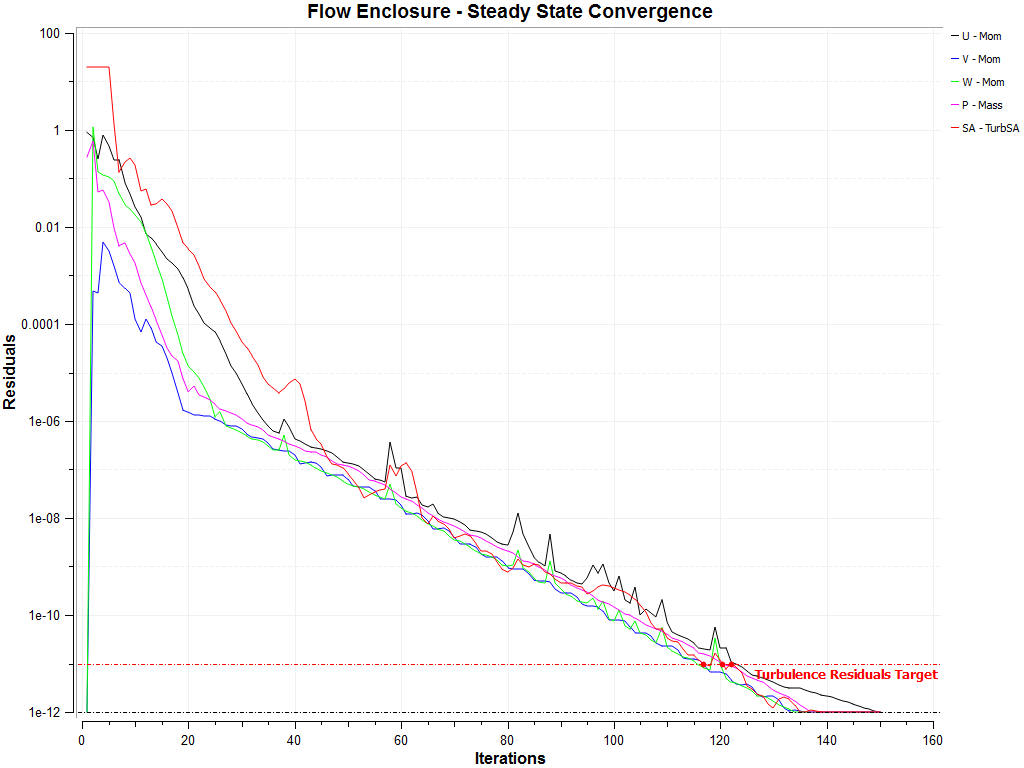
\includegraphics[width=\textwidth]{./figs/flatnx/35x25_conv.png}
        \caption{35x25}
    \end{subfigure}
    \hfill
    \begin{subfigure}{0.48\textwidth}
        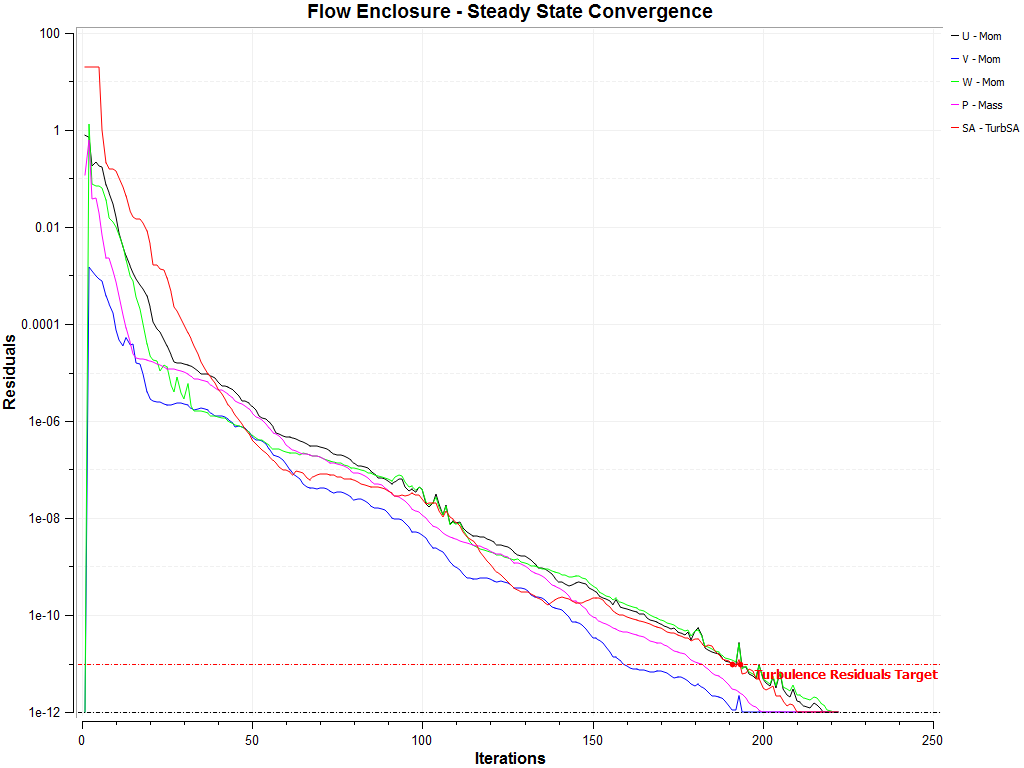
\includegraphics[width=\textwidth]{./figs/flatnx/69x49_conv.png}
        \caption{69x49}
    \end{subfigure}
    \\
    \begin{subfigure}{0.48\textwidth}
        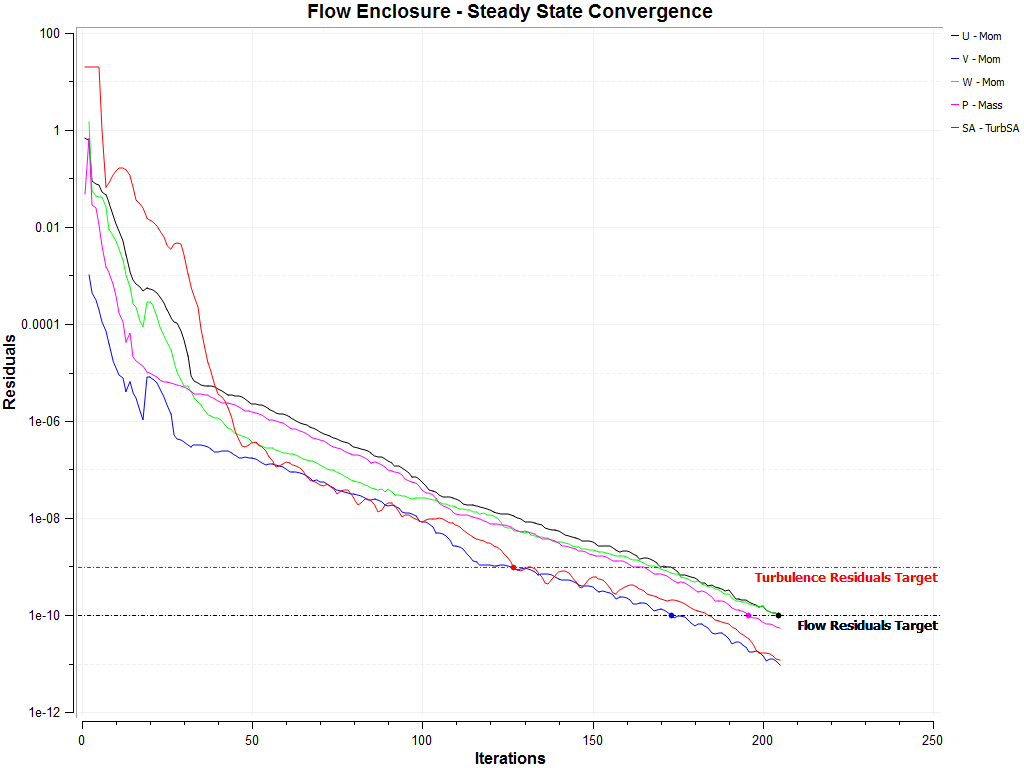
\includegraphics[width=\textwidth]{./figs/flatnx/137x97_conv.png}
        \caption{137x97}
    \end{subfigure}
    \hfill
    \begin{subfigure}{0.48\textwidth}
        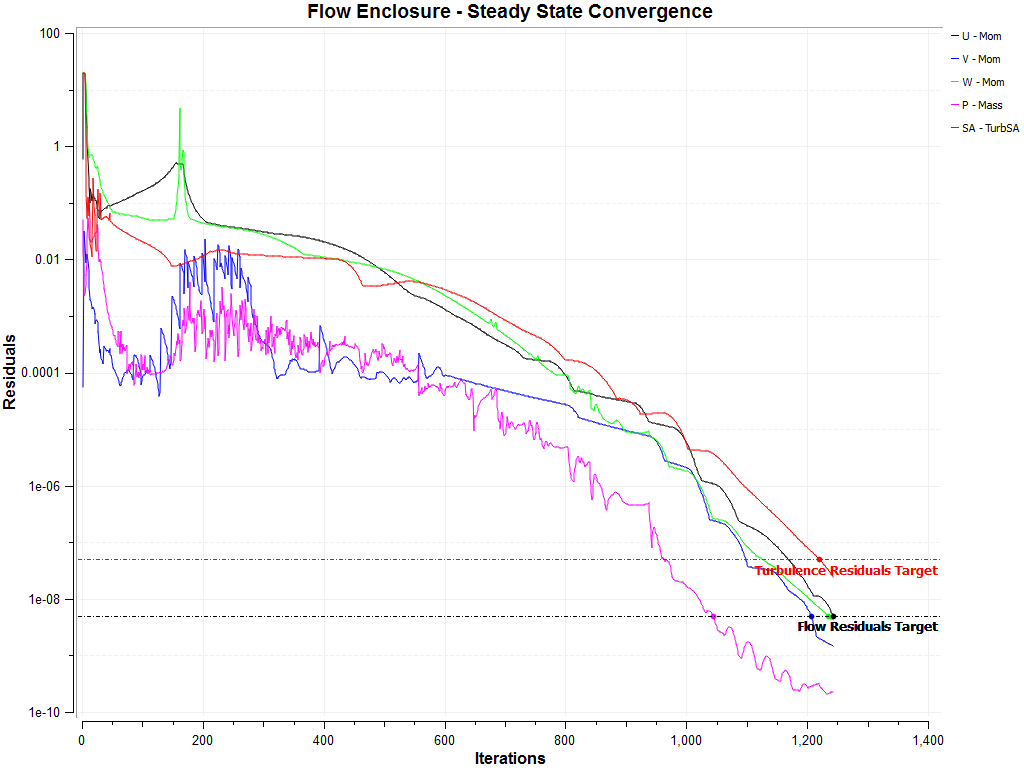
\includegraphics[width=\textwidth]{./figs/flatnx/273x193_conv.png}
        \caption{273x193}
    \end{subfigure}
    \\
    \begin{subfigure}{0.48\textwidth}
        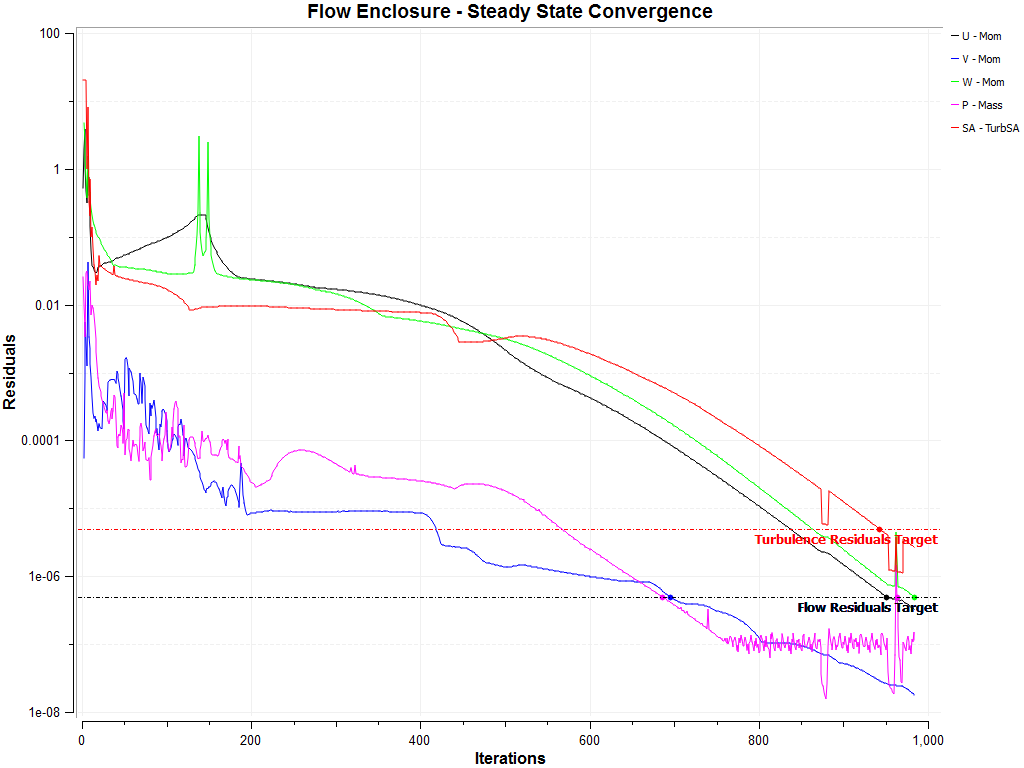
\includegraphics[width=\textwidth]{./figs/flatnx/545x385_conv.png}
        \caption{545x385}
    \end{subfigure}
    \caption{Flat Plate (NX Flow): Convergence of residuals on various grid sizes.}
    \label{fig:nxflatcnvstudy}
\end{figure}

Unless otherwise noted, all results were obtained with the finest grid. \Cref{fig:nxflatcf} compares the skin friction along the plate. \Cref{fig:nxflatmutcontour} shows contour plots of the dimensionless eddy viscosity and \Cref{fig:nxflatmu} shows line plots of the dimensionless eddy viscosity. \Cref{fig:nxflatu,fig:nxflatupyp} show profiles of the dimensionless velocity $u/u_\infty$ and $u^+$ respectively. Similarly to Syn3D, the eddy viscosity jumps abruptly right at the leading edge, as seen in~\Cref{fig:nxflatmutmax}. 
\begin{figure}[ht!]
\centering
	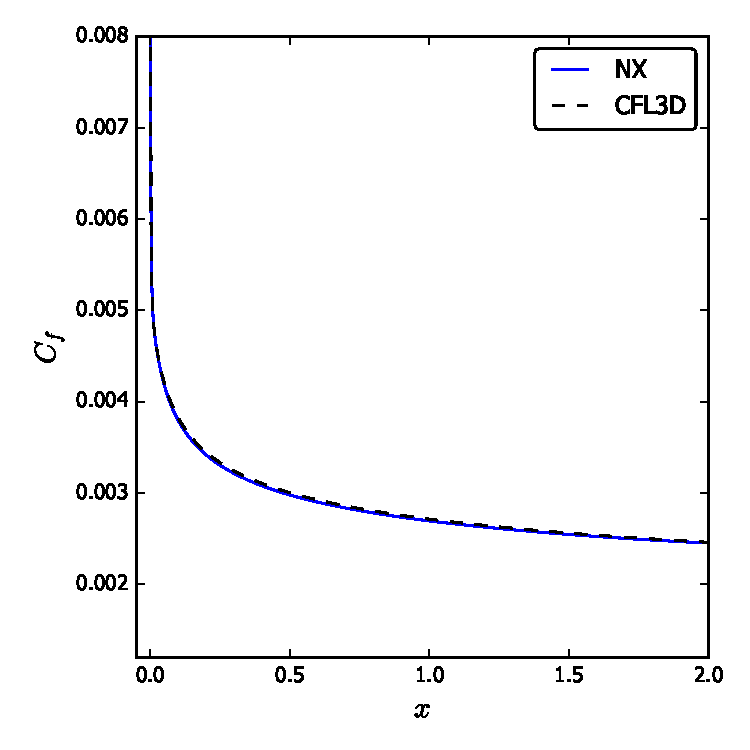
\includegraphics[width=0.7\textwidth]{figs/flatnx/cf.pdf}
    \caption{Flat Plate (NX Flow): Coefficient of skin friction along the plate.}
    \label{fig:nxflatcf}
\end{figure}

\begin{figure}[ht!]
\centering
\begin{subfigure}{.45\textwidth}
  \centering
  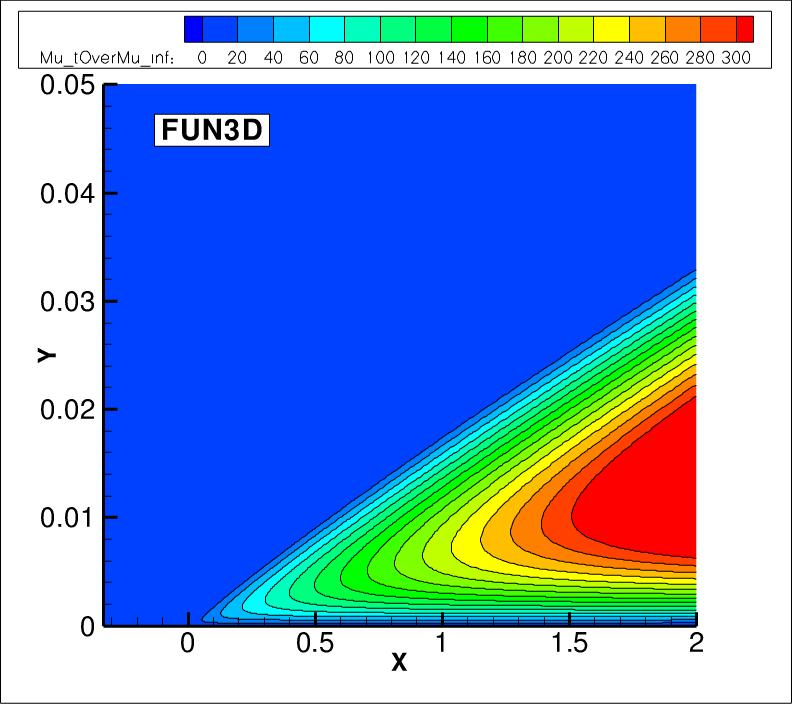
\includegraphics[width=1.0\textwidth]{figs/flatnx/mut_contour_fun3d.jpg}
  \caption{CFL3D}
\end{subfigure}%
\begin{subfigure}{.45\textwidth}
  \centering
  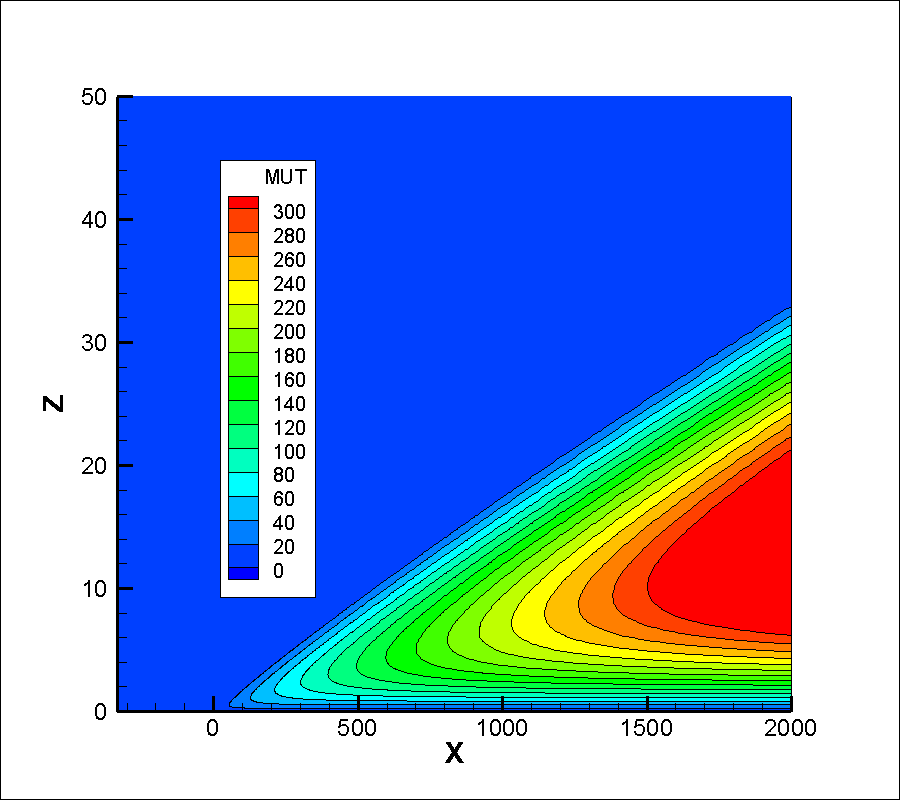
\includegraphics[width=1.0\textwidth]{figs/flatnx/mut_contour.png}
  \caption{NX Flow}
\end{subfigure}
\caption{Flat Plate (NX Flow): Contours of non-dimensionalized eddy viscosity}
\label{fig:nxflatmutcontour}
\end{figure}

\begin{figure}[ht!]
\centering
\begin{subfigure}{.45\textwidth}
  \centering
  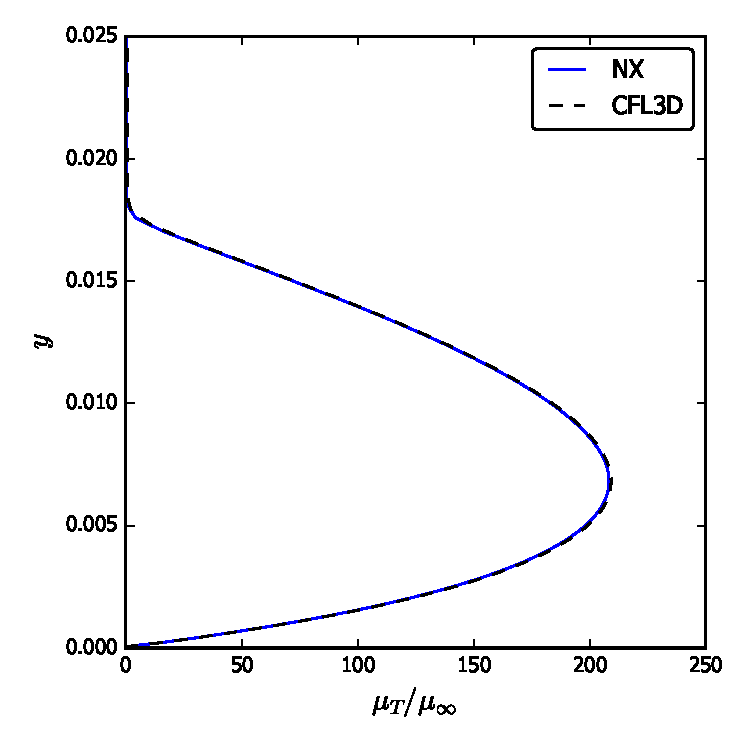
\includegraphics[width=1.0\textwidth]{figs/flatnx/mut.pdf}
  \caption{Nondimensional eddy viscosity at x=0.97 }
\end{subfigure}%
\begin{subfigure}{.45\textwidth}
  \centering
  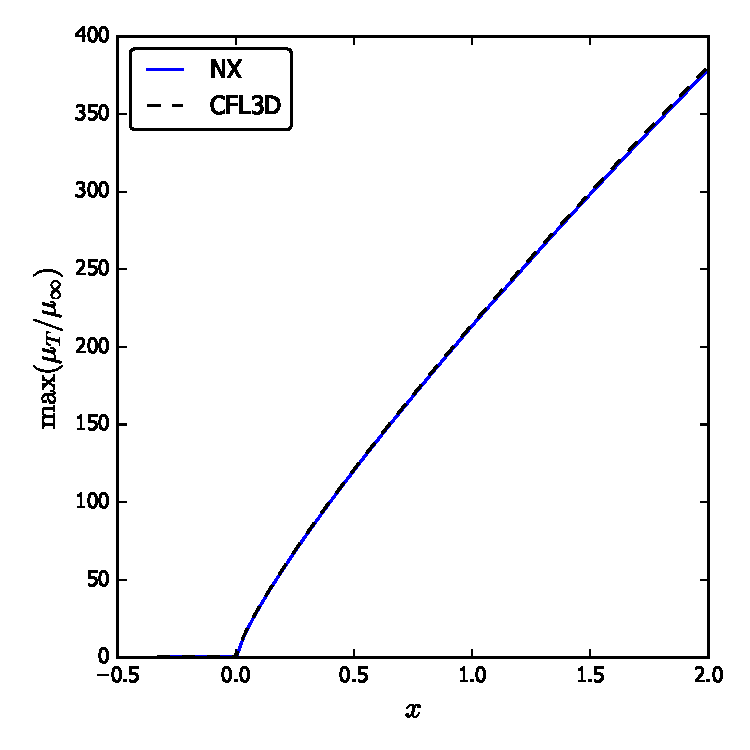
\includegraphics[width=1.0\textwidth]{figs/flatnx/maxmut.pdf}
  \caption{Maximum $\frac{\mu_t}{\mu_{\infty}}$ in the boundary layer}
  \label{fig:nxflatmutmax}
\end{subfigure}
\caption{Flat Plate (NX Flow): Dimensionless eddy viscosity line plots}
\label{fig:nxflatmu}
\end{figure}

\begin{figure}[ht!]
\centering
\begin{subfigure}{.45\textwidth}
  \centering
  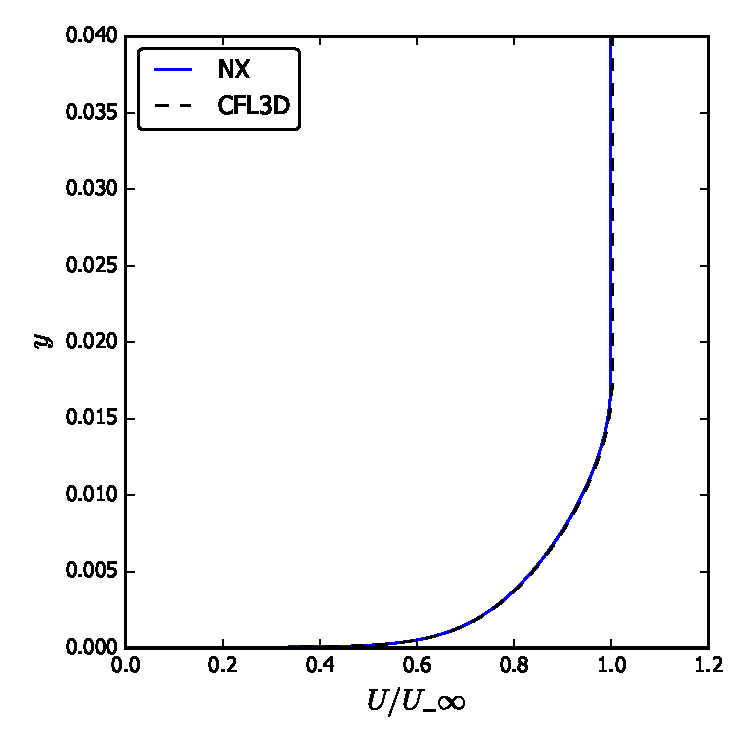
\includegraphics[width=1.0\textwidth]{figs/flatnx/u_x097.pdf}
  \caption{$x=0.97$}
\end{subfigure}%
\begin{subfigure}{.45\textwidth}
  \centering
  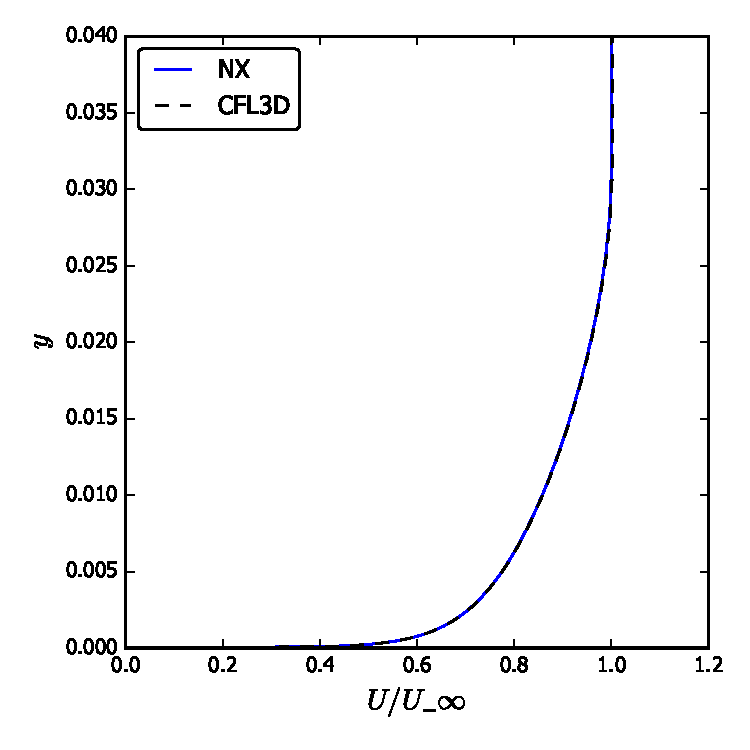
\includegraphics[width=1.0\textwidth]{figs/flatnx/u_x190.pdf}
  \caption{$x=1.90$}
\end{subfigure}
\caption{Flat Plate (NX Flow): $\frac{U}{U_{\infty}}$ profiles in the boundary layer}
\label{fig:nxflatu}
\end{figure}

\begin{figure}[ht!]
\centering
\begin{subfigure}{.45\textwidth}
  \centering
  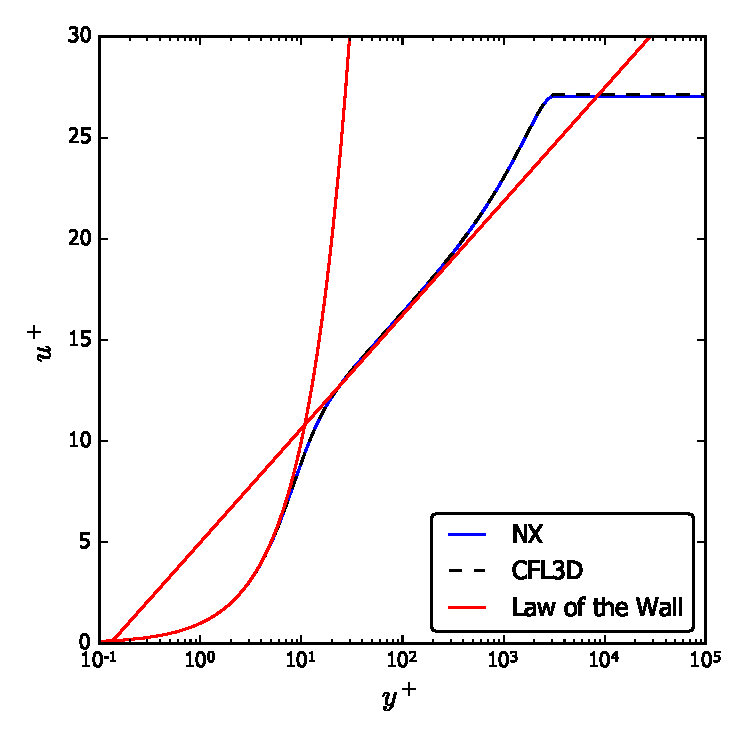
\includegraphics[width=1.0\textwidth]{figs/flatnx/uyplus_x097.pdf}
  \caption{$x=0.97$}
\end{subfigure}%
\begin{subfigure}{.45\textwidth}
  \centering
  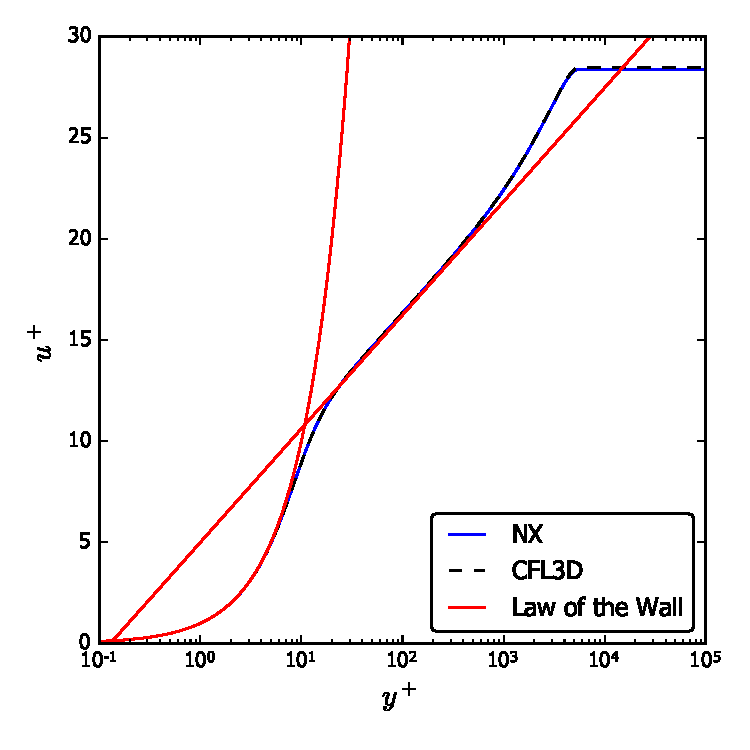
\includegraphics[width=1.0\textwidth]{figs/flatnx/uyplus_x190.pdf}
  \caption{$x=1.90$}
\end{subfigure}
\caption{Flat Plate (NX Flow): $u^+$ vs. $y^+$ profiles in the boundary layer. Law of the wall is also shown for comparison.}
\label{fig:nxflatupyp}
\end{figure}

\Cref{fig:nxflatforcestudy} shows the dependence of $C_D$ and $C_f$ on the grid spacing.  The results of running FUN3D in incompressible mode are also shown, and it can be seen that  \Cref{fig:nxflatcfstudy,fig:nxflatprofilestudy} show the variation of skin friction coefficient along the plate and profiles of eddy viscosity and velocity with grid size respectively. 
\begin{figure}[ht!]
\centering
\begin{subfigure}{.45\textwidth}
  \centering
  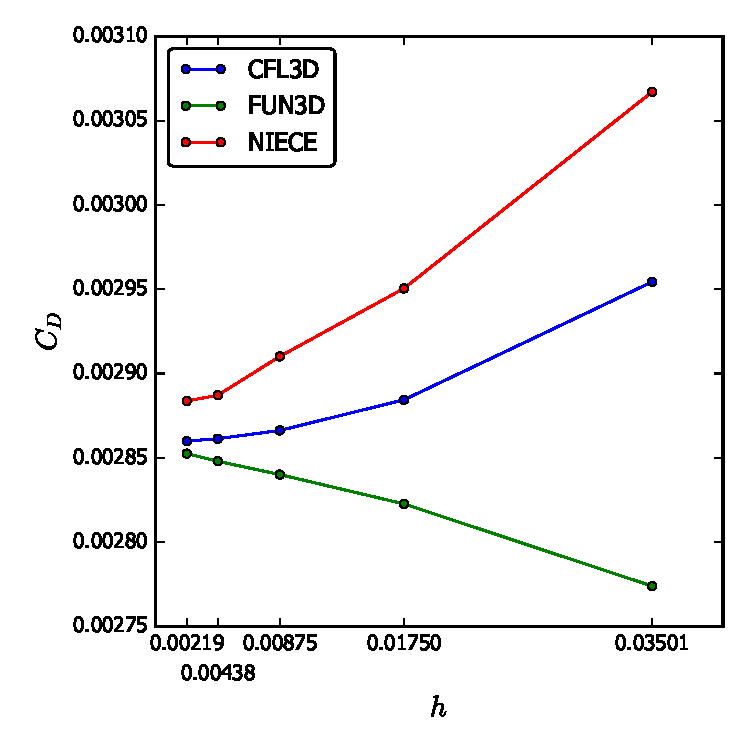
\includegraphics[width=1.0\textwidth]{figs/flatnx/cd_convergence.pdf}
  \caption{Coefficient of drag.}
\end{subfigure}%
\begin{subfigure}{.45\textwidth}
  \centering
  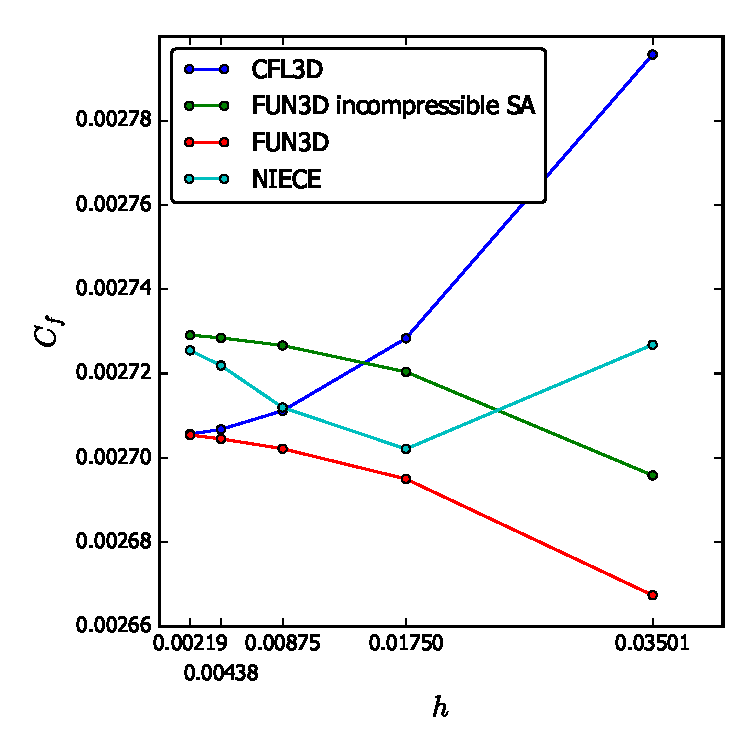
\includegraphics[width=1.0\textwidth]{figs/flatnx/cf_convergence.pdf}
  \caption{Coefficient of Skin Friction at x=0.97.}
\end{subfigure}
\caption{Flat Plate (NX Flow): Force coefficients for various grid sizes.}
\label{fig:nxflatforcestudy}
\end{figure}

\begin{figure}[ht!]
\centering
  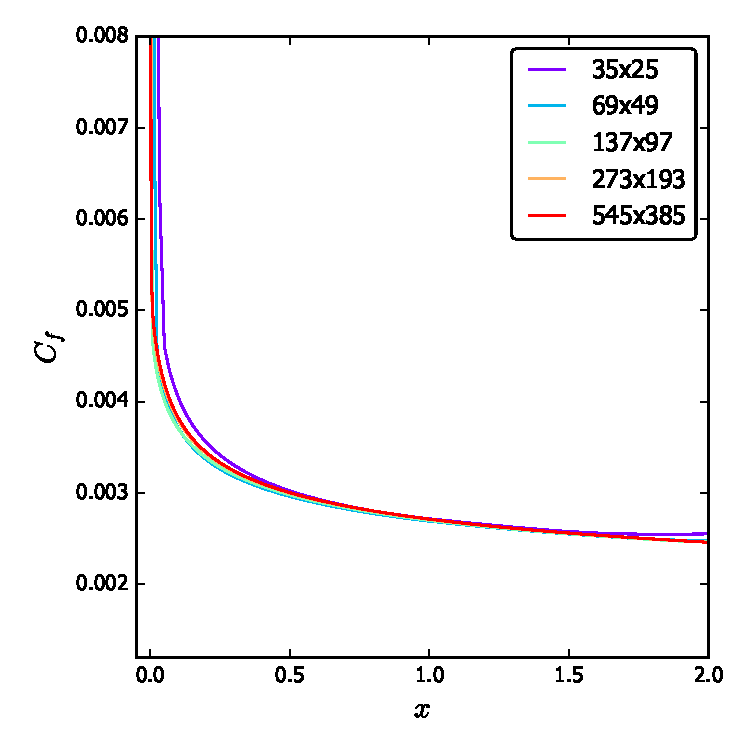
\includegraphics[width=0.7\textwidth]{figs/flatnx/cf_gridstudy.pdf}
  \caption{Flat Plate (NX Flow): Coefficient of skin friction on various grids.}
  \label{fig:nxflatcfstudy}
\end{figure}

\begin{figure}[ht!]
\centering
\begin{subfigure}{.45\textwidth}
  \centering
  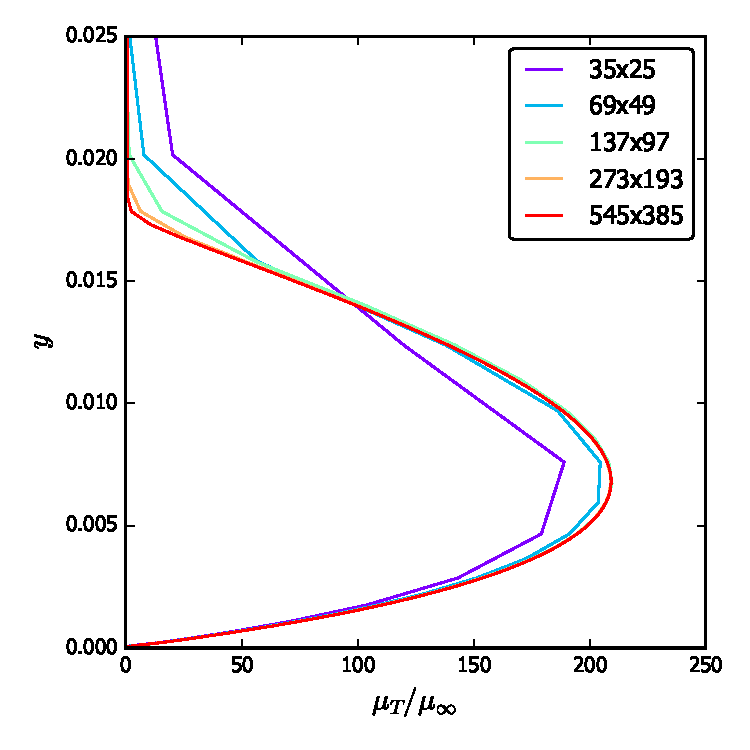
\includegraphics[width=1.0\textwidth]{figs/flatnx/mut_gridstudy.pdf}
  \caption{Dimensionless eddy viscosity}
\end{subfigure}%
\begin{subfigure}{.45\textwidth}
  \centering
  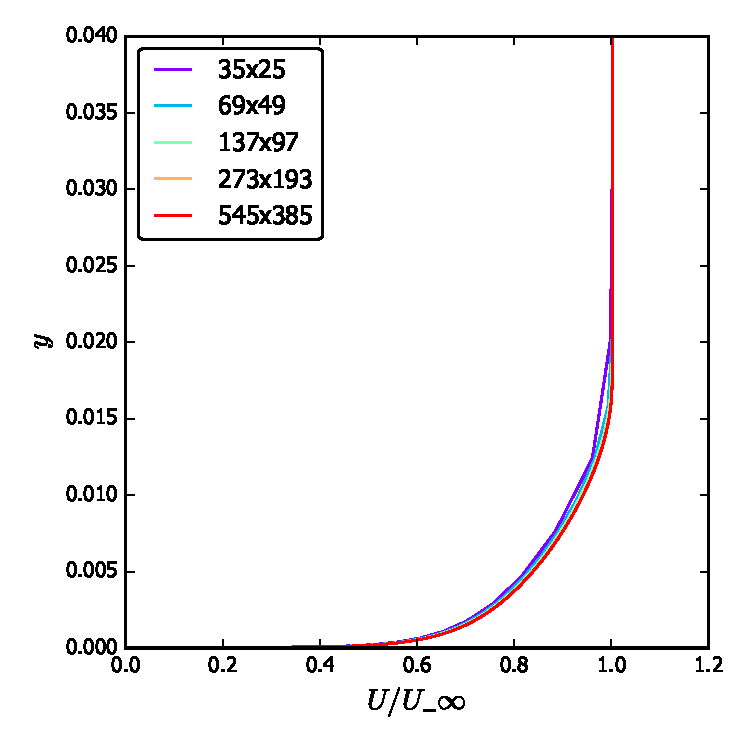
\includegraphics[width=1.0\textwidth]{figs/flatnx/u_x097_gridstudy.pdf}
  \caption{Dimensionless velocity}
\end{subfigure}
\caption{Flat Plate (NX Flow): Profiles at $x=0.97$ for various grid sizes.}
\label{fig:nxflatprofilestudy}
\end{figure}
